
 \documentclass[a4paper,12pt]{article}
%%%%%%%%%%%%%%%%%%%%%%%%%%%%%%%%%%%%%%%%%%%%%%%%%%%%%%%%%%%%%%%%%%%%%%%%%%%%%%%%%%%%%%%%%%%%%%%%%%%%%%%%%%%%%%%%%%%%%%%%%%%%%%%%%%%%%%%%%%%%%%%%%%%%%%%%%%%%%%%%%%%%%%%%%%%%%%%%%%%%%%%%%%%%%%%%%%%%%%%%%%%%%%%%%%%%%%%%%%%%%%%%%%%%%%%%%%%%%%%%%%%%%%%%%%%%
\usepackage{eurosym}
\usepackage{vmargin}
\usepackage{amsmath}
\usepackage[thinlines]{easytable}

\usepackage{enumerate}
\usepackage{multicol}
\usepackage{graphics}
\usepackage{epsfig}
\usepackage{framed}
\usepackage{subfigure}
\usepackage{fancyhdr}

\setcounter{MaxMatrixCols}{10}
%TCIDATA{OutputFilter=LATEX.DLL}
%TCIDATA{Version=5.00.0.2570}
%TCIDATA{<META NAME="SaveForMode" CONTENT="1">}
%TCIDATA{LastRevised=Wednesday, February 23, 2011 13:24:34}
%TCIDATA{<META NAME="GraphicsSave" CONTENT="32">}
%TCIDATA{Language=American English}

%\pagestyle{fancy}
\setmarginsrb{20mm}{0mm}{20mm}{25mm}{12mm}{11mm}{0mm}{11mm}
%\lhead{MA4413 2013} \rhead{Mr. Kevin O'Brien}
%\chead{Midterm Assessment 1 }
%\input{tcilatex}

\begin{document}

\section{Cluster Analysis}
\noindent \textbf{Objective:} create clusters of items, individuals or objects that have similarity with the others in the cluster but with differences between clusters.  
% Document prepared by Robert L. Andrews, April 2005 & revised, April 2011

\begin{itemize}
	\item The items, individuals or objects being placed into clusters will be referred to as cases.  The degree of similarity or dissimilarity may be determined from the recorded values for one or multiple characteristics for the cases.  There are no dependent variables for cluster analysis.  
\item Clustering procedures require that similarity be quantified.  One quantitative measure for interval scale data is the distance between cases.  Euclidean Distance measures the length of a straight line between two cases.  The numeric value of the distance between cases depends on the measurement scale.  
\item If the measurements are recorded using different measurement scales then one should use a transformation to assure similar variability of measurements for all characteristics being used to create the clusters (see Transform Values section below tell how this can be done in SPSS Hierarchical Cluster Analysis, otherwise this needs to be done prior to the analysis, for example, when using SPSS K-Means Cluster Analysis).  
\item Other measures may be used to create a dissimilarity or distance matrix that can be used as the basis for creating clusters (see Measures for Interval Data section under Hierarchical Cluster Analysis).  
	
\item A key issue in obtaining a set of clusters is the determination of the number of clusters.  Hierarchical procedures provide information that allows the analyst to decide on the number of clusters based on the output. 
\item  This is often done by examining tabular or graphical output to identify the gaps that define logical clusters.  The SPSS K-Means Cluster Analysis procedure requires that the number of clusters be specified to run the analysis. 
\item  The K-Means procedure is applicable for data sets with a large number of cases while the hierarchical procedure may be preferred when there are a limited number of cases.
\end{itemize}

\section{K-Means Clustering}
\begin{itemize}
	\item Hierarchical clustering requires a distance or similarity matrix between all pairs of cases. That's an extremely large matrix if you have tens of thousands of cases in your data file.
	
	\item A clustering method that doesn't require computation of all possible distances is k-means clustering. It differs from hierarchical clustering in several ways. You have to know in advance the number of clusters you want. You can't get solutions for a range of cluster numbers unless you rerun the analysis for each different number of clusters.
	
	\item The algorithm repeatedly reassigns cases to clusters, so the same case can move from cluster to cluster during the analysis. In agglomerative hierarchical clustering, on the other hand, cases are added only to existing clusters. They are forever captive in their cluster, with a widening circle of ``neighbours".
	
	\item The algorithm is called \textbf{k-means}, where \textbf{k} is the number of clusters you want, since a case is assigned to the cluster for which its distance to the cluster mean is the smallest.
	
	\item The k-means algorithm follows an entirely different concept than the hierarchical methods
	discussed before. This algorithm is not based on distance measures such as
	Euclidean distance or city-block distance, but uses the \textbf{\textit{within-cluster variation}} as a measure to form homogenous clusters. Specifically, the procedure aims at segmenting
	the data in such away that the within-cluster variation isminimized.Consequently,we
	do not need to decide on a distance measure in the first step of the analysis.
	
	\item The action in the algorithm centers around finding the k-means. You start out with an initial set of means and classify cases based on their distances to the centers.
	
	\item Next, you compute the cluster means again, using the cases that are assigned to the cluster; then, you reclassify all cases based on the new set of means. You keep repeating this step until cluster means don't change much between successive steps.
	
	\item Finally, you calculate the means of the clusters once again and assign the cases to their permanent clusters.
\end{itemize}
%------------------------------------------------------------------%
\subsection{Initial Cluster Centres}
The first step in k-means clustering is finding the k centres. This is done iteratively. You start with an initial set of centres and then modify them until the change between two iterations is small enough.

If you have good guesses for the centres, you can use those
as initial starting points; otherwise, you can let SPSS find k cases that are well separated and use these values as initial cluster centers. (i.e. The clustering process starts by randomly assigning objects to a number of
clusters).



K-means clustering is very sensitive to outliers, since they will usually be selected as initial cluster centers. This will result in outliers forming clusters with small numbers of cases. Before you start a cluster analysis, screen the data for outliers and remove them from the initial analysis. The solution may also depend on the order of the cases in the data.

After the initial cluster centers have been selected, each case is assigned to the closest
cluster, based on its distance from the cluster centers. After all of the cases have been
assigned to clusters, the cluster centers are recomputed, based on all of the cases in the
cluster.

The cases are then successively reassigned to other clusters to minimize the within-cluster variation, which is basically the (squared) distance from each observation to the center of the associated cluster. If the reallocation of an case to another cluster decreases the within-cluster variation, this case is reassigned
to that cluster.

Case assignment is done again, using these updated cluster centers. You keep
assigning cases and recomputing the cluster centers until no cluster center changes
appreciably or the maximum number of iterations (10 by default) is reached.
\newpage
\subsection{Demonstration of k-means}
In this example, two cluster centers are randomly
initiated, which CC1 (first cluster) and CC2 (second cluster).
\begin{figure}[h!]
	\begin{center}
		% Requires \usepackage{graphicx}
		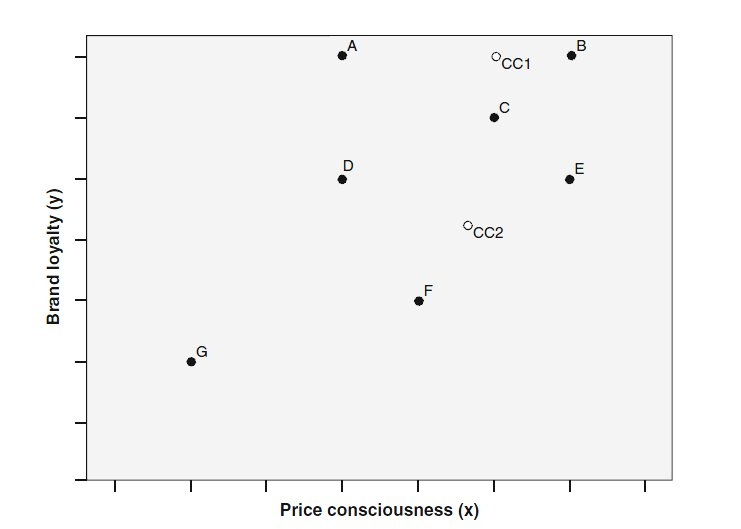
\includegraphics[scale=0.4]{images/kmeans1.jpg}\\
	\end{center}
\end{figure}
\begin{figure}[h!]
	\begin{center}
		% Requires \usepackage{graphicx}
		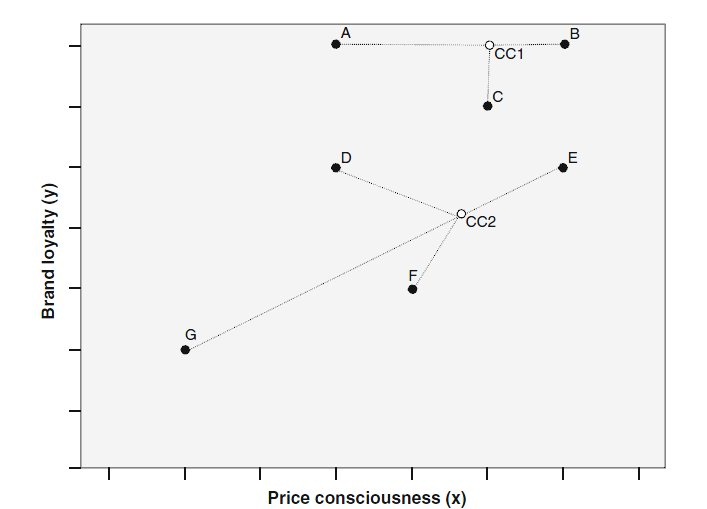
\includegraphics[scale=0.4]{images/kmeans2.jpg}\\
	\end{center}
\end{figure}
Euclidean distances are computed from the cluster
centers to every single object. Each object is then assigned to the cluster center with
the shortest distance to it.

In this example, objects A, B, and C are
assigned to the first cluster, whereas objects D, E, F, and G are assigned to the
second. We now have our initial partitioning of the objects into two clusters.
Based on this initial partition, each cluster’s geometric center (i.e., its centroid)
is computed (third step). This is done by computing the mean values of the objects
contained in the cluster (e.g., A, B, C in the first cluster) regarding each of the variables
(in this example: price consciousness and brand loyalty).
\begin{figure}[h!]
	\begin{center}
		% Requires \usepackage{graphicx}
		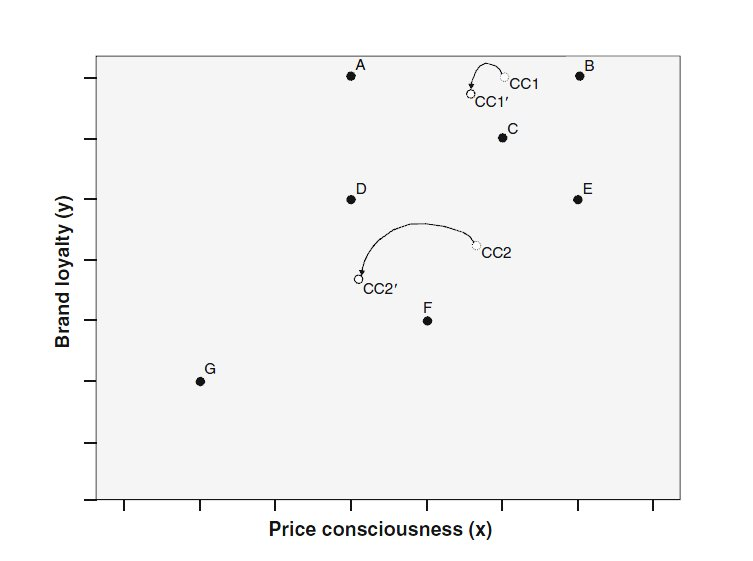
\includegraphics[scale=0.4]{images/kmeans3.jpg}\\
	\end{center}
\end{figure}
\begin{figure}[h!]
	\begin{center}
		% Requires \usepackage{graphicx}
		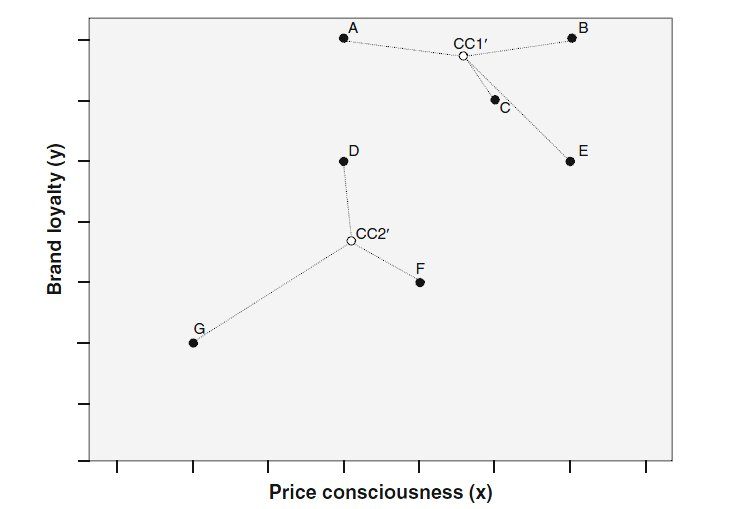
\includegraphics[scale=0.4]{images/kmeans4.jpg}\\
	\end{center}
\end{figure}
Both clusters’centers now shift into new positions (CC1’ for the first and CC2’ for the second cluster).
In the fourth step, the distances from each object to the newly located cluster
centers are computed and objects are again assigned to a certain cluster on the basis
of their minimum distance to other cluster centers (CC1’ and CC2’).

Since the cluster centers’ position changed with respect to the initial situation in the first step,
this could lead to a different cluster solution. This is also true of our example, as
object E is now – unlike in the initial partition – closer to the first cluster center
(CC1’) than to the second (CC2’). Consequently, this object is now assigned to the
first cluster.
The k-means procedure now repeats the third step and
re-computes the cluster centers of the newly formed clusters, and so on.
In other words, steps 3 and 4 are repeated until a predetermined number of iterations are
reached, or convergence is achieved (i.e., there is no change in the cluster affiliations).

\subsection{Performance of k-means clustering}
Generally, k-means is superior to hierarchical methods as it is less affected by
outliers and the presence of irrelevant clustering variables. Furthermore, k-means
can be applied to very large data sets, as the procedure is less computationally
demanding than hierarchical methods. In fact, we suggest definitely using k-means
for sample sizes above 500, especially if many clustering variables are used. From
a strictly statistical viewpoint, k-means should only be used on interval or ratio-scaled
data as the procedure relies on Euclidean distances. However, the procedure is
routinely used on ordinal data as well, even though there might be some distortions.

One problem associated with the application of k-means relates to the fact that
the researcher has to pre-specify the number of clusters to retain from the data. This
makes k-means less attractive to some and still hinders its routine application in
practice.

\section{Clustering Linkage Methods}

SPSS provides several alternative methods for determining a summary measure of distance when a cluster has multiple cases in the cluster.  The SPSS options for the clustering method are Between-groups linkage, Within-groups linkage, Nearest neighbor, Furthest neighbor, Centroid clustering, Median clustering, and Ward's method.

\begin{itemize}
\item For the \textbf{nearest neighbor} or \textbf{single linkage} method, the dissimilarity between cluster A and cluster B is represented by the minimum of all possible distances between the cases in cluster A and the cases in cluster B.

\item For the \textbf{furthest neighbor} or \textbf{complete linkage} method, the dissimilarity between cluster A and cluster B is represented by the maximum of all possible distances between the cases in cluster A and the cases in cluster B.

\item For the \textbf{between-groups linkage} or average linkage method, the dissimilarity between cluster A and cluster B is represented by the average of all the possible distances between the cases in cluster A and the cases in cluster B.

\item For the \textbf{within-groups linkage} method, the dissimilarity between cluster A and cluster B is represented by the average of all the possible distances between the cases within a single new cluster determined by combining cluster A and cluster B.
 
\item  
For the \textbf{centroid clustering} method, the dissimilarity between cluster A and cluster B is represented by the distance between the centroid for the cases in cluster A and the centroid for the cases in cluster B.  Note that this distance is not mathematically equivalent to the average of the distances used in the average linkage method.  Also note the SPSS warning below about using squared Euclidean distance rather than Euclidean distance for this procedure.

\begin{framed}
The squared Euclidean measure should be used when the CENTROID, MEDIAN, or WARD cluster method is requested.
\end{framed}

\item For \textbf{Ward’s method}, the dissimilarity between cluster A and cluster B is represented by the “loss of information” from joining the two clusters with this loss of information being measured by the increase in error sum of squares.  For a cluster the sum of squares is the sum of squared deviations of each case from the centroid for the cluster.  The error sum of squares is the total of these for all clusters.  When selecting clusters to join, the two clusters among all possible combinations that have the minimum increase in error sum of squares are selected.  See the note above about using squared Euclidean distance rather than Euclidean distance for this method.

\item 
For the \textbf{median clustering} method, the dissimilarity between cluster A and cluster B is represented by the distance between the SPSS determined median for the cases in cluster A and the median for the cases in cluster B.  See the message in the note above about using squared Euclidean distance rather than Euclidean distance for this method.

\end{itemize}

Cluster analysis can be an effective tool to identify extreme data values in a multivariate data set.  Extreme points will be a cluster by themselves while the vast majority of the other points are in one or more well populated clusters.  

When performing hierarchical cluster analysis one can cluster cases or variables in SPSS by selecting either cases or variables in the initial menu.  The default is cases since it is probably done more than clustering variables but clustering variables may be desirable in certain situations.  

 
 \newpage
\section*{Clustering Procedures: }
% (Descriptions below originally copied from SPSS13.0 Help & I have made % slight additions.)

\subsection*{Hierarchical Cluster Analysis}
This procedure attempts to identify relatively homogeneous groups of cases (or variables) based on selected characteristics, using an algorithm that starts with each case (or variable) in a separate cluster and combines clusters until only one is left. You can analyze raw variables or you can choose from a variety of standardizing transformations. Distance or similarity measures are generated by the Proximities procedure. Statistics are displayed at each stage to help you select the best solution.  Statistics include agglomeration schedule, distance (or similarity) matrix, and cluster membership for a single solution or a range of solutions.  Plots include dendrograms and icicle plots.
\begin{itemize}
	\item 	Agglomeration schedule. Displays the cases or clusters combined at each stage, the distances between the cases or clusters being combined, and the last cluster level at which a case (or variable) joined the cluster.
	\item 	Proximity matrix. Gives the distances or similarities between items.
	\item 	Cluster Membership. Displays the cluster to which each case is assigned at one or more stages in the combination of clusters. Available options are single solution and range of solutions.
	\item 	Dendrograms can be used to assess the cohesiveness of the clusters formed and can provide information about the appropriate number of clusters to keep.
	\item 	Icicle plots display information about how cases are combined into clusters at each iteration of the analysis. (User can specify a range of clusters to be displayed) Orientation allows you to select a vertical or horizontal plot.
\end{itemize}

\subsection*{Data.}  The variables can be quantitative, binary, or count data. Scaling of variables is an important issue--differences in scaling may affect your cluster solution(s). If your variables have large differences in scaling (for example, one variable is measured in dollars and the other is measured in years), you should consider standardizing them (this can be done automatically by the Hierarchical Cluster Analysis procedure).

\subsection*{Case Order.} If tied distances or similarities exist in the input data or occur among updated clusters during joining, the resulting cluster solution may depend on the order of cases in the file. You may want to obtain several different solutions with cases sorted in different random orders to verify the stability of a given solution.
\subsection*{Assumptions.}  The distance or similarity measures used should be appropriate for the data analyzed. Also, you should include all relevant variables in your analysis. Omission of influential variables can result in a misleading solution. Because hierarchical cluster analysis is an exploratory method, results should be treated as tentative until they are confirmed with an independent sample.



 \subsection*{Implementation}


To Obtain a Hierarchical Cluster Analysis
From the menus choose:
\begin{verbatim}
Analyze  >  Classify  >  Hierarchical Cluster...

\end{verbatim}
If you are clustering cases, select at least one numeric variable. If you are clustering variables, select at least three numeric variables. 


 
\subsection*{K-Means Cluster Analysis}
This procedure attempts to identify relatively homogeneous groups of cases based on selected characteristics, using an algorithm that can handle large numbers of cases. However, the algorithm requires you to specify the number of clusters. You can specify initial cluster centers if you know this information. You can select one of two methods for classifying cases, either updating cluster centers iteratively or classifying only. You can save cluster membership, distance information, and final cluster centers. Optionally, you can specify a variable whose values are used to label casewise output. You can also request analysis of variance F statistics. While these statistics are opportunistic (the procedure tries to form groups that do differ), the relative size of the statistics provides information about each variable's contribution to the separation of the groups.

Statistics. Complete solution: initial cluster centers, ANOVA table.  Each case: cluster information, distance from cluster center.


\subsection*{Implementation}

To Obtain a Hierarchical Cluster Analysis
From the menus choose:
\begin{verbatim}
Analyze  >  Classify  >  Hierarchical Cluster...

\end{verbatim}
If you are clustering cases, select at least one numeric variable. If you are clustering variables, select at least three numeric variables. 




\subsection*{Assumptions}
\begin{itemize}
	\item  Distances are computed using simple Euclidean distance. If you want to use another distance or similarity measure, use the Hierarchical Cluster Analysis procedure. Scaling of variables is an important consideration--if your variables are measured on different scales (for example, one variable is expressed in dollars and another is expressed in years), your results may be misleading.
	\item  In such cases, you should consider standardizing your variables before you perform the k-means cluster analysis (this can be done in the Descriptives procedure). The procedure assumes that you have selected the appropriate number of clusters and that you have included all relevant variables. 
	\item If you have chosen an inappropriate number of clusters or omitted important variables, your results may be misleading.
\end{itemize}


\subsection*{Case and Initial Cluster Center Order.} The default algorithm for choosing initial cluster centers is not invariant to case ordering. The Use running means option on the Iterate dialog box makes the resulting solution potentially dependent upon case order regardless of how initial cluster centers are chosen. If you are using either of these methods, you may want to obtain several different solutions with cases sorted in different random orders to verify the stability of a given solution. Specifying initial cluster centers and not using the Use running means option will avoid issues related to case order. However, ordering of the initial cluster centers may affect the solution, if there are tied distances from cases to cluster centers. Comparing results from analyses with different permutations of the initial center values may be used to assess the stability of a given solution.


\subsection*{Implementation}
To Obtain a K-Means Cluster Analysis
From the menus choose:
\begin{verbatim}
Analyze  >  Classify  >  K-Means Cluster...    
\end{verbatim}

\begin{itemize}
\item 	Select the variables to be used in the cluster analysis. 
\item 	Specify the number of clusters. The number of clusters must be at least two and must not be greater than the number of cases in the data file.
\item 	Select either Iterate and classify or Classify only.
\end{itemize}
\end{document}



=======
 \documentclass[a4paper,12pt]{article}
%%%%%%%%%%%%%%%%%%%%%%%%%%%%%%%%%%%%%%%%%%%%%%%%%%%%%%%%%%%%%%%%%%%%%%%%%%%%%%%%%%%%%%%%%%%%%%%%%%%%%%%%%%%%%%%%%%%%%%%%%%%%%%%%%%%%%%%%%%%%%%%%%%%%%%%%%%%%%%%%%%%%%%%%%%%%%%%%%%%%%%%%%%%%%%%%%%%%%%%%%%%%%%%%%%%%%%%%%%%%%%%%%%%%%%%%%%%%%%%%%%%%%%%%%%%%
\usepackage{eurosym}
\usepackage{vmargin}
\usepackage{amsmath}
\usepackage[thinlines]{easytable}

\usepackage{enumerate}
\usepackage{multicol}
\usepackage{graphics}
\usepackage{epsfig}
\usepackage{framed}
\usepackage{subfigure}
\usepackage{fancyhdr}

\setcounter{MaxMatrixCols}{10}
%TCIDATA{OutputFilter=LATEX.DLL}
%TCIDATA{Version=5.00.0.2570}
%TCIDATA{<META NAME="SaveForMode" CONTENT="1">}
%TCIDATA{LastRevised=Wednesday, February 23, 2011 13:24:34}
%TCIDATA{<META NAME="GraphicsSave" CONTENT="32">}
%TCIDATA{Language=American English}

%\pagestyle{fancy}
\setmarginsrb{20mm}{0mm}{20mm}{25mm}{12mm}{11mm}{0mm}{11mm}
%\lhead{MA4413 2013} \rhead{Mr. Kevin O'Brien}
%\chead{Midterm Assessment 1 }
%\input{tcilatex}

\begin{document}

\section{Cluster Analysis}
\noindent \textbf{Objective:} create clusters of items, individuals or objects that have similarity with the others in the cluster but with differences between clusters.  
% Document prepared by Robert L. Andrews, April 2005 & revised, April 2011

The items, individuals or objects being placed into clusters will be referred to as cases.  The degree of similarity or dissimilarity may be determined from the recorded values for one or multiple characteristics for the cases.  There are no dependent variables for cluster analysis.  Clustering procedures require that similarity be quantified.  One quantitative measure for interval scale data is the distance between cases.  Euclidean Distance measures the length of a straight line between two cases.  The numeric value of the distance between cases depends on the measurement scale.  If the measurements are recorded using different measurement scales then one should use a transformation to assure similar variability of measurements for all characteristics being used to create the clusters (see Transform Values section below tell how this can be done in SPSS Hierarchical Cluster Analysis, otherwise this needs to be done prior to the analysis, for example, when using SPSS K-Means Cluster Analysis).  Other measures may be used to create a dissimilarity or distance matrix that can be used as the basis for creating clusters (see Measures for Interval Data section under Hierarchical Cluster Analysis).  

A key issue in obtaining a set of clusters is the determination of the number of clusters.  Hierarchical procedures provide information that allows the analyst to decide on the number of clusters based on the output.  This is often done by examining tabular or graphical output to identify the gaps that define logical clusters.  The SPSS K-Means Cluster Analysis procedure requires that the number of clusters be specified to run the analysis.  The K-Means procedure is applicable for data sets with a large number of cases while the hierarchical procedure may be preferred when there are a limited number of cases.

\subsection*{Clustering Methods}

SPSS provides several alternative methods for determining a summary measure of distance when a cluster has multiple cases in the cluster.  The SPSS options for the clustering method are Between-groups linkage, Within-groups linkage, Nearest neighbor, Furthest neighbor, Centroid clustering, Median clustering, and Ward's method.

\begin{itemize}
\item For the \textbf{nearest neighbor} or \textbf{single linkage} method, the dissimilarity between cluster A and cluster B is represented by the minimum of all possible distances between the cases in cluster A and the cases in cluster B.

\item For the \textbf{furthest neighbor} or \textbf{complete linkage} method, the dissimilarity between cluster A and cluster B is represented by the maximum of all possible distances between the cases in cluster A and the cases in cluster B.

\item For the \textbf{between-groups linkage} or average linkage method, the dissimilarity between cluster A and cluster B is represented by the average of all the possible distances between the cases in cluster A and the cases in cluster B.

\item For the \textbf{within-groups linkage} method, the dissimilarity between cluster A and cluster B is represented by the average of all the possible distances between the cases within a single new cluster determined by combining cluster A and cluster B.
 
\item  
For the \textbf{centroid clustering} method, the dissimilarity between cluster A and cluster B is represented by the distance between the centroid for the cases in cluster A and the centroid for the cases in cluster B.  Note that this distance is not mathematically equivalent to the average of the distances used in the average linkage method.  Also note the SPSS warning below about using squared Euclidean distance rather than Euclidean distance for this procedure.

\begin{framed}
The squared Euclidean measure should be used when the CENTROID, MEDIAN, or WARD cluster method is requested.
\end{framed}

\item For \textbf{Ward’s method}, the dissimilarity between cluster A and cluster B is represented by the “loss of information” from joining the two clusters with this loss of information being measured by the increase in error sum of squares.  For a cluster the sum of squares is the sum of squared deviations of each case from the centroid for the cluster.  The error sum of squares is the total of these for all clusters.  When selecting clusters to join, the two clusters among all possible combinations that have the minimum increase in error sum of squares are selected.  See the note above about using squared Euclidean distance rather than Euclidean distance for this method.

\item 
For the \textbf{median clustering} method, the dissimilarity between cluster A and cluster B is represented by the distance between the SPSS determined median for the cases in cluster A and the median for the cases in cluster B.  See the message in the note above about using squared Euclidean distance rather than Euclidean distance for this method.

\end{itemize}

Cluster analysis can be an effective tool to identify extreme data values in a multivariate data set.  Extreme points will be a cluster by themselves while the vast majority of the other points are in one or more well populated clusters.  

When performing hierarchical cluster analysis one can cluster cases or variables in SPSS by selecting either cases or variables in the initial menu.  The default is cases since it is probably done more than clustering variables but clustering variables may be desirable in certain situations.  

 
 \newpage
\section*{Clustering Procedures: }
% (Descriptions below originally copied from SPSS13.0 Help & I have made % slight additions.)







To Obtain a K-Means Cluster Analysis
From the menus choose:
\begin{verbatim}
Analyze  >  Classify  >  K-Means Cluster...    
\end{verbatim}

\begin{itemize}
\item 	Select the variables to be used in the cluster analysis. 
\item 	Specify the number of clusters. The number of clusters must be at least two and must not be greater than the number of cases in the data file.
\item 	Select either Iterate and classify or Classify only.
\end{itemize}
\end{document}



